
%\documentclass[12pt]{article}
\documentclass{article}
%\documentclass[10pt]{article}

%\usepackage{mslapa}
\usepackage{hyperref}
\usepackage{amsmath}
\usepackage{graphicx}
\usepackage{ulem}
%\usepackage{vmargin}
\usepackage{tabularx}
\usepackage{sectsty}
\usepackage{pbox}
\usepackage{bigstrut}
\usepackage{enumerate}
\usepackage{listings}
\usepackage{parskip}   % space paragraphs but dont indent
\usepackage{verbatim}  % \verbatiminput{file}

%\usepackage{cleveref}

%\setpapersize{USletter}
\sectionfont{\normalsize}
\subsectionfont{\normalsize}

% configure \bigstrut size
% This configures spacing above and below rows in a tabularx.
%\renewcommand{\bigstrutjot}{6pt}
\renewcommand{\bigstrutjot}{2.0\jot}

\providecommand{\e}[1]{\ensuremath{\times 10^{#1}}}

%\setlength{\parindent}{0in}
%\setlength{\parindent}{1.5ex}
%\setlength{\parskip}{1ex plus 0.5ex minus 0.2ex}

\raggedright

\begin{document}

% If a figure is too long to fit in a figure on a single page
% it should got in its own section in the Appendix.

% {{{ Cover Page

\centerline{\bf EECE 311}
\centerline{\bf Fall 2011}
\centerline{\bf}
\centerline{\bf Lab Report \#4}
\centerline{\bf Modeling and Analyzing AC Circuits (RC and RL) with SPICE}
%\centerline{\bf Section 4}
%\centerline{\bf 9/13/2011} % date turned in
\centerline{\bf 10/4/2011}  % date lab performed
\centerline{\bf}

% signature area
\begin{center}
\begin{tabularx}{\textwidth}[b]{X l l}
Signature & Printed Name & Date \\
\hline
\multicolumn{1}{|X|}{} & \multicolumn{1}{|l|}{\bigstrut \bf Jeremiah Mahler} & \multicolumn{1}{|l|}{\bf Oct 11, 2011} \\
\hline
%\multicolumn{1}{|X|}{} & \multicolumn{1}{|l|}{\bigstrut \bf Marvanee Johnson} & \multicolumn{1}{|l|}{\bf Sep 14, 2011} \\
%\hline
\end{tabularx}
\end{center}
% }}}

% Following the instructions for section definitions in the Syllabus
% http://www.ecst.csuchico.edu/~hma/SYL.311.htm

% {{{ Objective
% Puropse of experiment
\section{Objective}

% objective take from lab instructions
The objective of this labratory exercise is to learn and gain
experience analyzing and simulating the behavior of first
order RC and RL circuits under transient conditions using a SPICE simulator.

% }}}

% {{{ Equipment
\section{Equipment}

To perform the circuit simulation the Ngspice\cite{NGSPICE} SPICE\cite{wiki:SPICE} simulator was used.
Other SPICE simulators such as Pspice\cite{wiki:Pspice} and Orcad\cite{ORCAD}
should work as well.

%\clearpage
% }}}

% {{{ Procedure
\section{Procedure}

Two circuits will be analyzed; one is an RC with a capacitor and
the other is an RL with a inductor.
For each of these circuits this experiment consists of two main steps.
\begin{enumerate}
\item Build a SPICE definition of the circuit.
\item Run the simulation and record the output.
\end{enumerate}

In general a SPICE simulation can be run using Ngspice with the command
\begin{verbatim}
  ngspice -b your_file.cir
\end{verbatim}
where \verb+your_file.cir+ replaced by the name of your file
containing the SPICE definition.
To save the output to a file a redirect can be used as in:
\begin{verbatim}
  ngspice -b your_file.cir > your_file.out
\end{verbatim}

% {{{ RC Circuit
\subsection{RC Circuit}

The RC circuit to be analyzed is shown in Figure \ref{fig:rccircuit}.
The SPICE definition is shown in Figure \ref{fig:spice_rc}.

\begin{figure}[!hbtp]
\center
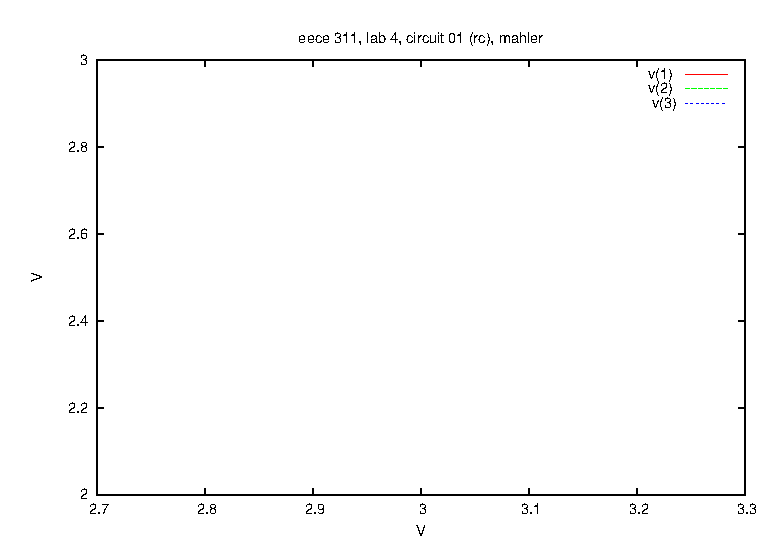
\includegraphics[scale=0.5]{spice/rc_circuit-01}
\caption{RC Circuit definition.
Nodes denoted by numbers with 0 as common.
V1 is a voltage source, I1 is a current source.
For the current source I1, $u(t)$ is the unit step function
which has a value of $0$ until $t > 0$.
This causes the current source to change from 0 amps to 6 mA at $t = 0$.
}
\label{fig:rccircuit}
\end{figure}

\begin{figure}[!hbtp]
\verbatiminput{spice/rc_circuit-01.cir}
\caption{SPICE definition of RC circuit in Figure \ref{fig:rccircuit}.}
\label{fig:spice_rc}
\end{figure}

% ensure all the figures for this section are displayed in this section
\clearpage

% }}}

% {{{ RL circuit
\subsection{RL circuit}

The RL circuit to be analyzed is shown in Figure \ref{fig:rlcircuit}.
The SPICE definition is shown in Figure \ref{fig:rlspice}.

\begin{figure}[!hbtp]
\center
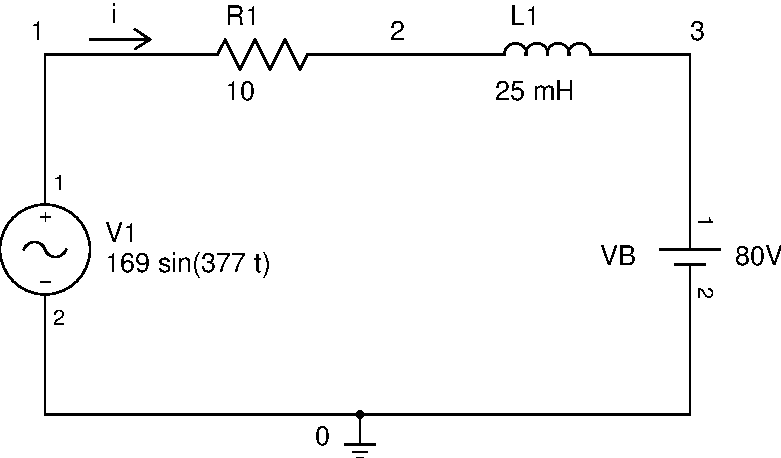
\includegraphics[scale=0.5]{spice/rl_circuit-01}
\caption{RL Circuit definition.
Nodes denoted by numbers with 0 as common.
V1 is an alternating current voltage source, VB is a direct current
voltage source, L1 is an inductor.}
\label{fig:rlcircuit}
\end{figure}

\begin{figure}[!hbtp]
\verbatiminput{spice/rl_circuit-01.cir}
\caption{SPICE definition of RL circuit in Figure \ref{fig:rlcircuit}.}
\label{fig:rlspice}
\end{figure}

% }}}

\clearpage
% }}}

% {{{ Results
\section{Results}

% {{{ RC circuit results
\subsection{RC circuit}

The output of the SPICE simulation of the RC circuit (Figure \ref{fig:rccircuit})
is shown in Figure \ref{fig:plot1}.

\begin{figure}[!hbtp]
\center
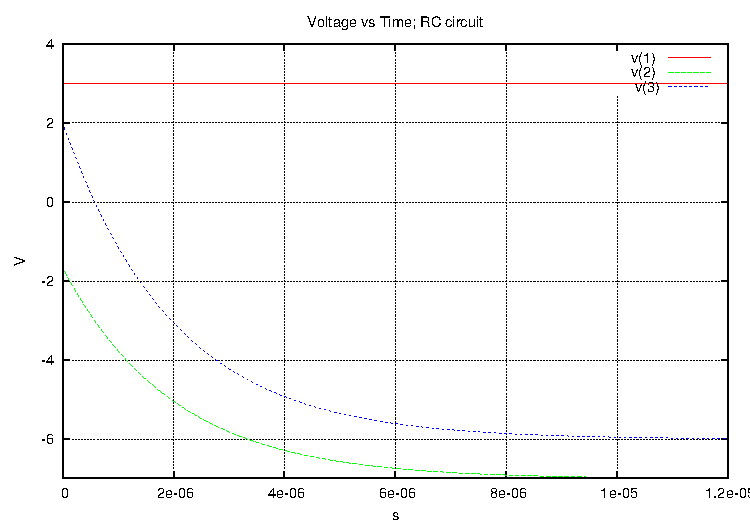
\includegraphics[scale=1.0]{spice/plot-01}
\caption{Plot of SPICE simultaion (Figure \ref{fig:spice_rc}) for
the RC circuit (Figure \ref{fig:rccircuit}).
The change of the current source from zero current to 6 mA
results in charging of the capacitor.
The voltage is negative as a result of the sign orientation used
in the circuit.}
\label{fig:plot1}
\end{figure}
\nocite{GNUPLOT}

\clearpage
% }}}

% {{{ RL circuit results
\subsection{RL circuit}

The output of the SPICE simulation of the RL circuit (Figure \ref{fig:rlcircuit})
is shown in Figure \ref{fig:rlplot1}.

\begin{figure}[!hbtp]
\center
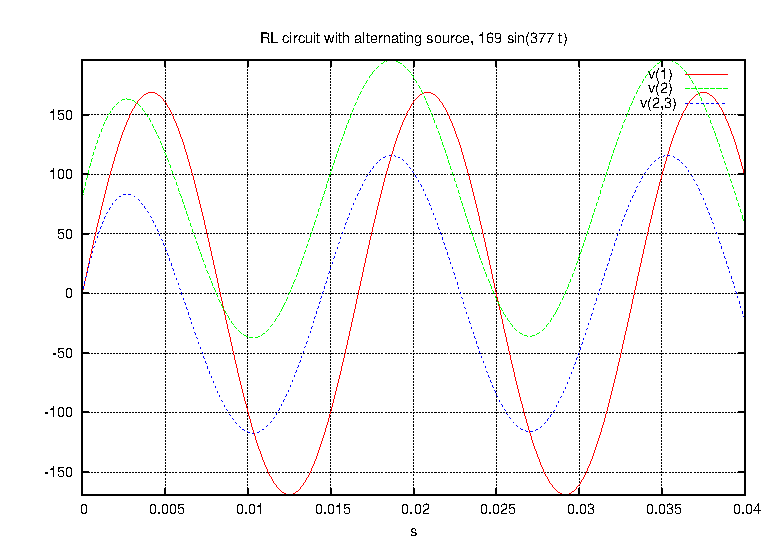
\includegraphics[scale=1.0]{spice/rlplot-01}
\caption{Plot of SPICE simultaion (Figure \ref{fig:rlspice}) for
the RL circuit (Figure \ref{fig:rlcircuit}).
Notice that during the first cycle it has not yet reached the steady
state because the amplitude is lower than during subsequent cycles.
The voltage across the inductor ($v(2,3)$) is offset compared to the
alternating voltage source ($v_1$) and is shifted due to
the DC voltage source ($v_B$).}
\label{fig:rlplot1}
\end{figure}
\nocite{GNUPLOT}

\clearpage
% }}}

% }}}

% {{{ Correlation with theory
\section{Correlation with theory}

To correlate the simulation with theory manual calculations are performed.

% {{{ RC circuit
\subsection{RC circuit}

The first stage of analysis is to determine the steady state conditions
at $t = 0^-$, before the circuit before switch point of the
unit step function ($u(t)$).
Referring to Figure \ref{fig:rccircuit}, it can be seen that when the current
source is flowing 0 amps the open circuit voltage across the capacitor
can be calculated as a voltage divider.

\begin{align*}
	v_3(0^-) &= 3 \cdot \frac{6k}{6k + 2k + 1k} \\
			&= 2.0 \quad \mbox{[volts]}
\end{align*}

The second stage is to simplify the circuit in to an equivalent
circuit with only one resistor, one capacitor and one voltage source.
Figure \ref{fig:rccircuiteq} shows the result of this simplification.

\begin{figure}[!hbtp]
\center
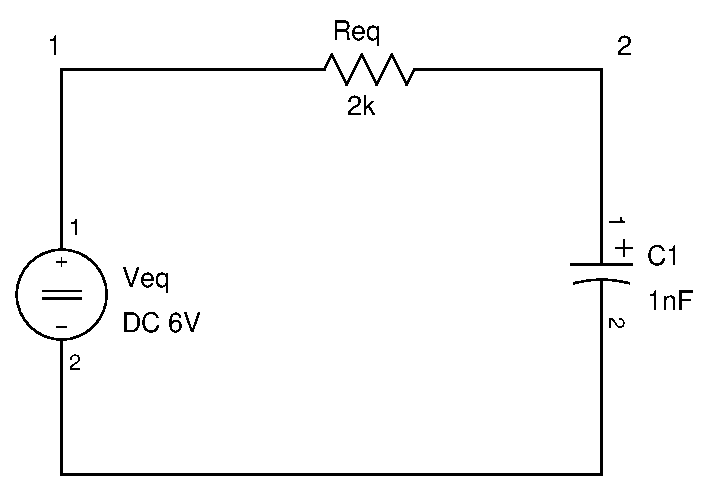
\includegraphics[scale=0.5]{spice/rc_circuit-02}
\caption{Simplified form of RC circuit from Figure \ref{fig:rccircuit}}
\label{fig:rccircuiteq}
\end{figure}

Using the simplified circuit (Figure \ref{fig:rccircuiteq})
along with Kirchoff's voltage law and the equation for a capacitor
the behavior of the circuit is given by Equation \ref{eq:rc1}.

\begin{align}
	6 + R C \frac{dv}{dt} + v &= 0  \label{eq:rc1}
\end{align}
And solving this first order differential equation:
\begin{align*}
	-R C \frac{dv}{dt} &= 6 + v \\
	-R C \frac{dv}{v + 6} &= dt \\
	\int_{v(0)}^{v(t)} \frac{dv}{v + 6} &= -\frac{1}{RC} \int_0^t dt \\
	-\frac{t}{RC} &= \left[ \ln (v(t) + 6) - \ln(v(0) + 6) \right] \\
	-\frac{t}{RC} &= \ln \left( \frac{v(t) + 6)}{v(0) + 6} \right) \\
	e^{-t/(RC)} &= \frac{v(t) + 6)}{v(0) + 6} \\
	v(t) + 6 &= (v(0) + 6) e^{-t/(RC)} \\
	v(t) &= -6 + (v(0) + 6) e^{-t/(RC)}
\end{align*}

And substituting the actual parameters along with the initial voltage:
\begin{align}
	v(t) &= -6 + (2.0 + 6) e^{-t \; 500\e{3}} \quad \mbox{[volts]} \notag \\
	v(t) &= -6 + 8 e^{-t \; 500\e{3}} \quad \mbox{[volts]}  \label{eq:rc2}
\end{align}

Next, values are substituted in to Equation \ref{eq:rc2} and compared to
the plot (Figure \ref{fig:plot1}).
As $t$ goes to $\infty$ the voltage across the capacitor goes to $-6$ volts.
At $t = 0$ the voltage across the capacitor is 2.0 volts.
At an arbitrary point, $t = 2 R C$, the voltage across the capacitor is -4.92 volts.
All these values agree with the plot from the SPICE simulation.

% }}}

% {{{ RL circuit
\subsection{RL circuit}

There are two possible ways two analyze the RL circuit with an alternating
voltage source.
The first is by using differential equations.
This is the most complex method but it completely describes the behavior
including transient conditions.
The second is to analyze only during steady state conditions
\cite[Pg. 330]{nilsson2008electric},
This method uses the concept of impedance and is much simpler but excludes
the transient conditions.
To simplify this analysis the second method will be used.

First the impedances of each passive circuit element is found.

\begin{align*}
	Z_{R1} &= 10 \\
	Z_{L1} &= j \omega L \\
		   &= j 9.425 \\
	Z_{eq} &= Z_{R1} + Z_{L1} \\
			&= 10 + j 9.425
\end{align*}

Since the effect of the DC voltage source ($v_B$) only serves
to shift the voltage it will not be included in the intermediate calculations.
It will be accounted for at the end.

The voltage source must be converted to the complex plane.

\begin{align*}
	V_1 &= 169 \sin(377 t) \\
		&= 169 \cos(377 t - 90) \\
		&= 169 \cos(377 t - \pi/2) \\
		&= 169 \angle -90^{\circ} \\
		&= 0 - j 169
\end{align*}

The current is found in the complex plane by using the voltage ($V_1$) and
the equivalent impedance ($Z_{eq}$).

\begin{align*}
	I &= \frac{V_1}{Z_{eq}} \\
		&= \frac{0 - j169}{10 + j 9.425} \\
		&= -8.435 - j 8.949
\end{align*}

The voltage across the inductor is found using the current ($I$) and
the impedance ($Z_L$).

\begin{align}
	V_L &= I Z_L \notag \\
		&= (-8.435 - j 8.949)(j 9.425) \notag \\
		&= 84.35 - j 7.950 \notag \\
		&= 115.913 \angle -43.30^{\circ} \notag \\
		&= 115.913 \cos(377t - 43.30^{\circ}) \notag \\
		&= 115.913 \cos(377t - 0.756) \notag
\end{align}

And to find the voltage at node $2$ the DC voltage source is added back in.

\begin{align}
	V_2 &= V_L + V_B \notag \\
	V_2 &= 115.913 \cos(377t - 0.756) + 80  \label{eq:rlvl} 
\end{align}

Equation \ref{eq:rlvl} describes the voltage at node 2 ($V_2$)
over time.
Substituting for various arbitrary values:
at $t = 0.01875$ $V_2 = 115.86$, at $t = 0.01$ $V_2 = -114.971$.
These values agree approximately with the plot of SPICE output (Figure \ref{fig:rlplot1}).

%\clearpage
% }}}

% }}}

% {{{ Conclusion
\section{Conclusion}

This experiment was a success in analyzing the behavior of first order
RC and RL circuits under transient conditions.
The calculated values approximately matched the plotted values from
the SPICE output and agreed with the theory.

% }}}

% {{{ References
%\clearpage

%\pagebreak
\renewcommand*{\refname}{\vspace{-8mm}}
\section{References}
\bibliographystyle{ieeetr}
\bibliography{../references}
% }}}

\end{document}

% vim:foldmethod=marker

